
\documentclass[a4paper]{article}
\usepackage[pdftex]{graphicx}
\usepackage[utf8]{inputenc}
\usepackage{enumerate}
\usepackage{siunitx}
\sisetup{locale=DE} 
\usepackage{icomma}
\usepackage{amssymb}
\usepackage{tikz}
\usepackage{href-ul}
\hypersetup{
	colorlinks=true,
	linkcolor=blue,
	urlcolor=blue}
\usepackage{geometry}
\geometry{a4paper, top=15mm, left=15mm, right=15mm, bottom=15mm,
	headsep=10mm, footskip=12mm}


\begin{document}
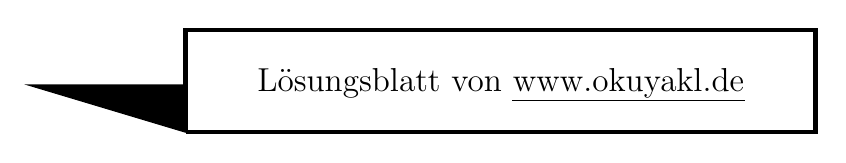
\begin{tikzpicture}(10,3)
	\draw[ultra thick](2,0) --(10,0) -- (10,1.3) --(2,1.3) -- (2,0);
	\draw[fill=black](2,0)-- (0,.6) -- (2,.6) -- (2,0);
	\node at (6,.6) {\large Lösungsblatt von \href{https://www.okuyakl.de}{www.okuyakl.de}};
\end{tikzpicture}
\vspace{0.5 cm}


\noindent
\begin{minipage}{0.5\textwidth}
	\bf{Aufgabe 1. a)}\\
	\includegraphics[width=5 cm]{wike96.pdf}
\end{minipage}
\hfill
\begin{minipage}{0.5\textwidth}
	\bf{Aufgabe 1. b)}\\
	\includegraphics[width=5 cm]{wili96.pdf}
\end{minipage}

\begin{tabular}{c|c|c|c|c|c|c|c|c|c}
	& $U$ in $\SI{}{\volt}$ & 0 & 0,30 & 0,60 & 0,90 & 1,20 & 1,50 & 1,80 & 2,10 \\
	\hline
	Eisendraht            & $I$ in $\SI{}{\ampere}$ & 0 & 0,48 & 0,93 & 1,38 & 1,70 & 1,98 & 2,19 & 2,31 \\
	& $R$ in $\SI{}{\ohm}$ & 0 & 0,63 & 0,65 & 0,65 & 0,70 & 0,76 & 0,82 & 0,91  \\
	\hline
	Konstantandraht  & $I$ in $\SI{}{\ampere}$ & 0 & 0,09 & 0,18 & 0,27 & 0,36 & 0,45 & 0,54 & 0,63 \\
		& $R$ in $\SI{}{\ohm}$ & 0 & 3,33 & 3,33 & 3,33  & 3,33 & 3,33 & 3,33 & 3,33 \\
		\hline
\end{tabular}
\vspace{10 pt}

\noindent{\bf{Aufgabe 1. c)}}\\
Die Leiterkennlinie von Eisen verläuft oberhalb derjenigen von Konstantan. Daraus folgt, dass der Eisendraht besser leitet. Vergleicht man die Form der beiden Kurven, so fällt auf, dass die Steigung der Konstantan-Linie überall gleich ist, die Eisenkennlinie jedoch steil ansteigt und mit steigender Stromstärke flacher wird. 
Bei steigender Stromstärke erhitzen sich jedoch beide Drähte. Dies bedeutet, dass Konstantan in warmem wie im kaltem Zustand gleich gut leitet, Eisen mit steigender Temperatur schlechter. Dies belegen auch die berechneten Widerstandswerte in der Tabelle.
\vspace{0.5 cm}

\noindent{\bf{Aufgabe 1. d)}}\\
Der elektrische Widerstand von Eisen steigt mit der Temperatur. Die Ladungsträger sind reichlich vorhanden. Ihre möglichst geradlinige Bewegung von einem Pol zum anderen wird mit zunehmender Eigenbewegung der Atomrümpfe gestört.
\vspace{0.5 cm}

\noindent{\bf{Aufgabe 2.}}\\
Der zusätzliche Widerstand muss den größeren Stromfluss am Messgerät vorbei leiten, also parallel geschaltet werden. Der Widerstandswert des sogenannten Shunts berechnet sich folgendermaßen:

Zunächst berechnen wir die am Strommessgerät anliegende Spannung bei Vollausschlag:
$$U_{max} = R \cdot I = \SI{3,0}{\milli\ampere} \cdot \SI{70}{\ohm} = \SI{0,21}{\volt}$$
Diese Spannung muss nun auch am Ampèremeter anliegen, wenn $$I_V=\SI{30}{\milli\ampere}-\SI{3,0}{\milli\ampere}=\SI{27}{\milli\ampere}$$ 
durch den Shunt an ihm vorbeifließen. Dann gilt für dessen Widerstand: $R_S$:
$$R_S= {U_{max} \over I_V}={\SI{0,21}{\volt} \over \SI{0,027}{\ampere}}= \SI{7,8}{\ohm}$$
\vspace{0.5 cm}

\noindent{\bf{Aufgabe 3.}}\\
Mit einem Innenwiderstand kann man rechnen wie mit einem gewöhnlichen Widerstand. Am Innenwiderstand der Starterbatterie fällt folgende Spannung ab:
$$U_i= I \cdot R_i = \SI{120}{\ampere} \cdot \SI{0,030}{\ohm}= \SI{3,6}{\volt}$$
Diese Spannung ist von der Quellenspannung abzuziehen, um die Betriebsspannung $U_B$ zu erhalten:
$$ U_B = \SI{12}{\volt} - \SI{3,6}{\volt} = \SI{8,4}{\volt}$$
Damit erhalten wir für den Widerstand $R_A$ des Anlassers:
$$ R_A = {U_B \over I} = {\SI{8,4}{\volt} \over \SI{120}{\ampere}}=\SI{0,07}{\ohm}$$

\vspace{0.5 cm}

\noindent{\bf{Aufgabe 4. a)}}\\

\noindent
\begin{minipage}{0.6\textwidth}
	Kleinste Leistung:\\
	\includegraphics[width=10 cm]{wrei96.pdf}
\end{minipage}
\hfill
\begin{minipage}{0.4\textwidth}
	Größte Leistung:\\
	\includegraphics[width=5 cm]{wpar96.pdf}
\end{minipage}
\vspace{0.5 cm}

\noindent{\bf{Aufgabe 4. b)}}\\
Kleinste Leistung = größter Widerstand = Reihenschaltung:
$$R_{rei}= \SI{50}{\ohm} + \SI{50}{\ohm} + \SI{50}{\ohm} = \SI{150}{\ohm} $$
$$P_{rei}= U \cdot I = U \cdot {U\over R} = {U^2 \over R} = {(\SI{230}{\volt})^2 \over \SI{150}{\ohm}}= \SI{353}{\watt}$$
Größte Leistung = kleinster Widerstand = Parallelschaltung:
$$R_{par}= \left( {1\over \SI{50}{\ohm}} + {1\over\SI{50}{\ohm}} + {1\over \SI{50}{\ohm}} \right)^{-1} = {50 \over 3}\SI{}{\ohm} = \SI{16,7}{\ohm} $$
$$P_{par}={(\SI{230}{\volt})^2 \over \SI{16,7}{\ohm}}= \SI{3170}{\watt}$$

\begin{center}
	\includegraphics[width=7 cm]{../../viecher/endcomic.pdf}
	
	Hier geht es zurück zum \href{https://www.okuyakl.de/phys/p10elL096/aa096.pdf}{Aufgabenblatt}
\end{center}

\end{document}